\newpage
\subsection{Caso d'uso UC10 - Visualizzazione API registrate}
\label{UC10}
\begin{figure}[ht]
	\centering
	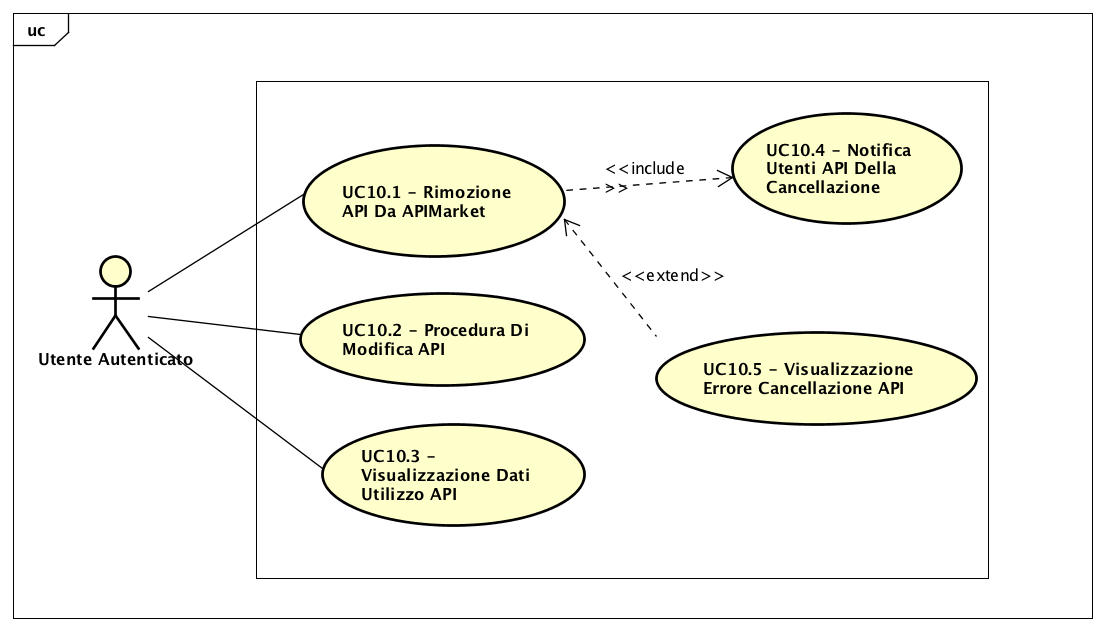
\includegraphics[scale=0.45]{UML/UC10.png}
	\caption{UC10: Visualizzazione API registrate}
\end{figure}

\begin{longtable}{ l | p{11cm}}
	\hline
	\rowcolor{Gray}
	\multicolumn{2}{c}{UC10 - Visualizzazione API registrate}\\
	\hline
	
	 \textbf{Attori} & Utente autenticato  \\
	\textbf{Descrizione} & L'attore può visualizzare la schermata relativa alle API da lui registrate \\
	\textbf{Pre-Condizioni} & L'attore seleziona il link per visualizzare le API registrate  \\
	\textbf{Post-Condizioni} & L'attore visualizza la pagina relativa alle API da lui registrate\\
	\textbf{Scenario Principale} & 
	\begin{enumerate*}[label=(\arabic*.),itemjoin={\newline}]
		\item L'attore visualizza il numero di API registrate (UC10.1)
		\item L'attore visualizza la lista di API registrate (UC10.2)
	\end{enumerate*}\\
	\textbf{Scenari Alternativi} & 
	\begin{enumerate*}[label=(\arabic*.),itemjoin={\newline}]
		\item L'attore può visualizzare i dati relativi a una singola API (UC7)
	\end{enumerate*}\\
\end{longtable}


\subsubsection{Caso d'uso UC10.1: Visualizzazione numero API registrate}
\label{UC10_1}

\begin{minipage}{\linewidth}
	\begin{tabular}{ l | p{11cm}}
		\hline
		\rowcolor{Gray}
		\multicolumn{2}{c}{UC10.1 - Visualizzazione numero API registrate} \\
		\hline
		\textbf{Attori} & Utente autenticato \\
		\textbf{Descrizione} & L'attore visualizza il numero di API da lui registrate nella schermata relativa\\
		\textbf{Pre-Condizioni} & L'attore si trova nel menù relativo alle API da lui registrate\\
		\textbf{Post-Condizioni} & L'attore visualizza il numero di API registrate \\
		\textbf{Scenario Principale} & 
		\begin{enumerate*}[label=(\arabic*.),itemjoin={\newline}]
			\item L'attore può visualizzare il numero di API da lui registrate nella piattaforma
		\end{enumerate*}\\
	\end{tabular}
\end{minipage}

\subsubsection{Caso d'uso UC10.2: Visualizzazione lista API registrate}
\label{UC10_2}

\begin{minipage}{\linewidth}
	\begin{tabular}{ l | p{11cm}}
		\hline
		\rowcolor{Gray}
		\multicolumn{2}{c}{UC10.2 - Visualizzazione lista API registrate} \\
		\hline
		\textbf{Attori} & Utente autenticato \\
		\textbf{Descrizione} & L'attore visualizza la lista di API da lui registrate nella schermata relativa\\
		\textbf{Pre-Condizioni} & L'attore si trova nel menù relativo alle API da lui registrate\\
		\textbf{Post-Condizioni} & L'attore visualizza la lista di API registrate \\
		\textbf{Scenario Principale} & 
		\begin{enumerate*}[label=(\arabic*.),itemjoin={\newline}]
			\item L'attore visualizza il nome dell'API (10.2.1)
			\item L'attore visualizza il link alla pagina dell'API (10.2.2)
			\item L'attore visualizza il numero di licenze attive (10.2.3)
		\end{enumerate*}\\
	\end{tabular}
\end{minipage}

\paragraph{Caso d'uso UC10.2.1: Visualizzazione nome API}
\label{UC10_2_1}

\begin{minipage}{\linewidth}
	\begin{tabular}{ l | p{11cm}}
		\hline
		\rowcolor{Gray}
		\multicolumn{2}{c}{UC10.2.1 - Visualizzazione nome API} \\
		\hline
		\textbf{Attori} & Utente autenticato \\
		\textbf{Descrizione} & L'attore visualizza il nome dell'API\\
		\textbf{Pre-Condizioni} & L'attore visualizza la lista API nel menù relativo alle API da lui registrate\\
		\textbf{Post-Condizioni} & L'attore visualizza il nome dell'API nella lista \\
		\textbf{Scenario Principale} & 
		\begin{enumerate*}[label=(\arabic*.),itemjoin={\newline}]
			\item L'attore può visualizzare il nome dell'API
		\end{enumerate*}\\
	\end{tabular}
\end{minipage}

\paragraph{Caso d'uso UC10.2.2: Visualizzazione link API}
\label{UC10_2_2}

\begin{minipage}{\linewidth}
	\begin{tabular}{ l | p{11cm}}
		\hline
		\rowcolor{Gray}
		\multicolumn{2}{c}{UC10.2.2 - Visualizzazione link API} \\
		\hline
		\textbf{Attori} & Utente autenticato \\
		\textbf{Descrizione} & L'attore visualizza il link dell'API\\
		\textbf{Pre-Condizioni} & L'attore visualizza la lista API nel menù relativo alle API da lui registrate\\
		\textbf{Post-Condizioni} & L'attore visualizza il link dell'API nella lista \\
		\textbf{Scenario Principale} & 
		\begin{enumerate*}[label=(\arabic*.),itemjoin={\newline}]
			\item L'attore può visualizzare il link dell'API
		\end{enumerate*}\\
	\end{tabular}
\end{minipage}

\paragraph{Caso d'uso UC10.2.3: Visualizzazione numero licenze attive}
\label{UC10_2_3}

\begin{minipage}{\linewidth}
	\begin{tabular}{ l | p{11cm}}
		\hline
		\rowcolor{Gray}
		\multicolumn{2}{c}{UC10.2.3 - Visualizzazione numero licenze attive} \\
		\hline
		\textbf{Attori} & Utente autenticato \\
		\textbf{Descrizione} & L'attore visualizza il numero di licenze attive per ogni voce della lista\\
		\textbf{Pre-Condizioni} & L'attore visualizza la lista API nel menù relativo alle API da lui registrate\\
		\textbf{Post-Condizioni} & L'attore visualizza il numero delle API vendute e attualmente attive \\
		\textbf{Scenario Principale} & 
		\begin{enumerate*}[label=(\arabic*.),itemjoin={\newline}]
			\item L'attore può visualizzare il numero delle API vendute e attualmente attive
		\end{enumerate*}\\
	\end{tabular}
\end{minipage}
